\documentclass{article}
\usepackage[utf8]{inputenc}
\usepackage[T1]{fontenc}
\usepackage{geometry}
\usepackage{graphicx}
\usepackage{natbib}
\usepackage{color}
\usepackage{type1ec}
\usepackage{authblk}
\usepackage{hyperref}
\usepackage{multirow}
\usepackage{booktabs}
\usepackage{setspace}
\RequirePackage{amsfonts,amsmath,amssymb,amsthm}
\newgeometry{top=3cm,bottom=2.2cm,left=3cm,right=3cm}


% \journal{Journal of BioSystems}

\begin{document}

\setcounter{page}{47}

\title{miRNAfe: a comprehensive tool for feature extraction in microRNA prediction}
\date{}
\author[1]{Cristian A. Yones\thanks{cyones@sinc.unl.edu.ar}}
\author[1]{Georgina Stegmayer}
\author[2]{Laura Kamenetzky}
\author[1]{Diego H. Milone}
\affil[1]{\small Research Institute for Signals, Systems and Computational Intelligence, sinc(i), FICH-UNL, CONICET, Ciudad Universitaria UNL, (3000) Santa Fe,
Argentina.}
\affil[2]{\small Instituto de Investigaciones en Microbiolog{\'i}a y Parasitolog{\'i}a M{\'e}dica (UBA), CONICET, Paraguay 2155, piso 13 (1121), Buenos Aires,
Argentina.}

\maketitle

\begin{abstract}
miRNAfe is a comprehensive tool to extract features from RNA sequences. It is freely available as a web service, allowing a single access point to almost all
state-of-the-art feature extraction methods used today in a variety of works from different authors. It has a very simple user interface, where the user only
needs to load a file containing the input sequences and select the features to extract. As a result, the user obtains a text file with the features extracted,
which can be used to analyze the sequences or as input to a miRNA prediction software.

The tool can calculate up to 80 features where many of them are multidimensional arrays. In order to simplify the web interface, the features have been divided
into six pre-defined groups, each one providing information about: primary sequence, secondary structure, thermodynamic stability, statistical stability,
conservation between genomes of different species and  substrings analysis of the sequences. Additionally, pre-trained classifiers are provided for prediction
in different species. All algorithms to extract the features have been validated, comparing the results with the ones obtained from software of the original
authors.

The source code is freely available for academic use under GPL license at \url{http://sourceforge.net/projects/sourcesinc/files/mirnafe/0.90/}. A user-friendly
access is provided as web interface at \url{http://fich.unl.edu.ar/sinc/web-demo/mirnafe/}. A more configurable web interface can be accessed at
\url{http://fich.unl.edu.ar/sinc/web-demo/mirnafe-full/}.
\end{abstract}

\textit{keywords: microRNA, Feature extraction, Web tool}


\section{Introduction}
MicroRNAs (miRNA) are a group of short ($\sim22$ nucleotides) non-coding RNA which can play important roles in gene regulation by targeting mRNAs for cleavage
or translational repression \citep{Lamers14}. Precursors of miRNA (pre-miRNA) are characterized by their hairpins structure. However, a large amount of similar
sequences can be folded into this kind of structure in many genomes.

In order to predict miRNAs, a large number of tools have been developed in the last years \citep{Kleftogiannis13}. The first step is to extract features from
sequences and then use classifiers to predict which sequences are likely to contain a miRNA. The feature extraction step is very important for the whole
process, in order to achieve high rates of true positives predictions \citep{Zhang10}.
Numerous features can be extracted from the primary sequence and its corresponding secondary structure. A typical example of this kind of features is the
\textit{triplets} representation \citep{Xue05}, which considers the structural composition of three adjacent nucleotides and the middle base to build a vector
with 32 elements. Other examples are the number of internal loops and their length \citep{Yousef06}, the z-score of the minimum free energy \citep{Hertel06}
and the dinucleotide proportion \citep{Rukshan09}. The amount of features that can be extracted is very large and there are many different tools that partially
achieve this task. They are coded in different programming languages and have different access modes (web, command line, etc.). Besides, several tools are
proprietary software and the source code is not even available\footnote{http://www.insybio.com/pages/ncrnaseq}. These are important issues that hinder their
use.

We have developed the miRNAfe tool that implements almost all existing state-of-the-art feature extraction processes used for miRNA prediction nowadays
\citep{Li10}. It can extract the features used by the most cited miRNA classifiers, such as Triplet-SVM \citep{Xue05}, RNAmicro \citep{Hertel06},
BayesMiRNAfind \citep{Yousef06}, MiRFinder \citep{Huang07}, MiPred \citep{Jiang07}, miRRim \citep{Goro07}, microPred \citep{Rukshan09}, miRanalyzer
\citep{Hackenberg09}, MiRenSVM \citep{Jiandong10} and miPredGA \citep{Xuan11}. We have developed an easy to use web interface that allows a single and
simplified access point to all the functions of the toolbox, and a set of pre-trained classifiers that can be used to test the prediction power of the feature
sets. We provide here a comprehensive open-source solution, with free access to all features for academic use.

\section{Provided features}

The tool implements up to 80 features, where many of them return arrays. All of these features have been proposed in literature over the past 10 years. The
features are divided into six pre-defined groups according to the kind of information that must be extracted from the sequence. A brief explanation of each
group is provided in the next lines. For a more detailed explanation of all the features provided and their sources, see the supplementary material.

\subsection{Sequence}
These are the simplest features and represent information from the primary sequence. MiRNAfe can extract a total of 5 features in this group: sequence length
($\ell$),  proportion of each base in the sequence, proportion of dinucleotides, content of guanine and cytosine and guanine-cytosine ratio. The last two
features are defined as:

\begin{equation} \label{eq:GCcontent}
 {G+C}_{content} = \frac{G+C}{G+C+A+U},
\end{equation}

\begin{equation} \label{eq:GCratio}
 {GC}_{ratio} = \frac{G}{C},
\end{equation}


\noindent where $G$, $C$, $A$ and $U$ represent the quantity of each base found in the sequence \citep{Hertel06}. All these features form a vector of 23
elements, composed by: the 4 base proportions, the 16 dinucleotide proportions, sequence length, ${G+C}_{content}$ and ${GC}_{ratio}$. Although these features
are quite simple, they have shown a high discriminative power \citep{Rukshan09}, and thus are used in most of the state-of-the-art prediction software.

\subsection{Secondary structure}
These features represent information from the secondary structure and they are the most numerous group. The most used feature of this group is the triplets
proportion \citep{Xue05}. A triplet is an element formed with the structure state (paired or not paired) of three adjacent nucleotides and the base at the
middle. An example of a triplet element is ``.((A'', where the parenthesis represents a paired nucleotide, a dot a not paired one, and the letter is the base
of the nucleotide in the middle. As there are 2 possible states for a nucleotide and 4 different bases, 32 triplets can be formed ($4 \times 2^{3}$). The
number of occurrences of each triplet element in the sequence is counted and normalized to produce a 32-­dimensional feature vector. A similar approach to the
triplets was used by \cite{Huang07}, which proposed another representation for the secondary structure. First of all, five symbols are defined to indicate the
status of each base pair in the stem: ``$=$'', ``$:$'', ``$-$'', ``$.$'' and ``$\wedge$''. Each of them corresponds to the status of match, mismatch, deletion,
insertion in the interior loop, and insertion in the bulged loop, respectively. Then, by taking two adjacent symbols, 14 possible combinations can be formed,
each one having a special meaning. For example: ``$=-$'', ``$=.$'', and ``$=:$'' represent the boundary of the stem/loop, and ``$:\wedge$'' represents that the
loop is asymmetric. The frequency of each combination is used as a feature vector. This representation is also used to calculate four more features: $pMatch$,
$pMismatch$, $pDI$ and $pBulge$. These features are calculated over putative mature miRNA, selected as the 22 nucleotide region where base-pairing is maximum.
They represents the base pairing frequency, the non-pairing frequency, the deletion and insertion frequencies and the symmetry of the bulged loops,
respectively.
%6 features

Another kind of features is related to the stems, which are structural motifs containing more than three contiguous base pairs \citep{Ng07}. These features are
the number of stems, the proportion of each possible base pair per stem, average base pair number per stem and length of the longest stem. %6 features
The rest of features are the stem region (the stem part of the stem-loop) length, terminal loop length, bulges number, loops number, longest loop length,
asymmetric and symmetric loops number, nucleotides in symmetric and asymmetric loops, longest symmetric region, average length of symmetric loops, average
length of asymmetric loops, number of bulges and loops of length $1,2,...,7$ and greater, base pair number, adjusted base pair propension, base pair proportion
and  $G+C_{content}$ in the terminal loop \citep{Lopes2014}. %20
Finally, miRNAfe can calculate reads count from RNAseq data. This feature needs the user to provide an extra file with reads, which miRNAfe aligns with the
analyzed sequences and counts the corresponding matches. For a full description of each feature see the supplementary material. %1

\subsection{Thermodynamics stability}
The features in this group are related to the thermodynamics stability of a sequence. The mostly used feature is the minimum free energy ($MFE$): the estimated
energy that one sequence frees when folded into the most stable secondary structure \citep{Zuker81}. The ensemble free energy ($EFE$) has a similar meaning and
it is obtained with the algorithm from \cite{McCaskill90}. Other features of this group are calculated as combinations of those values. For example, the MFE
index 1 ($MFEI_{1}$) is the ratio between the minimum free energy and the ${G+C}_{content}$ defined in \ref{eq:GCcontent}. Similarly, miRNAfe can calculate
$MFE-EFE$ difference, adjusted $MFE$, $MFEI_{2}$, $MFEI_{3}$ and $MFEI_{4}$ \citep{Rukshan09}. There are also some features that use information theoretic
approaches to estimate the confidence of the predicted secondary structure, such as the adjusted Shannon entropy of the pairing probabilities \citep{Ng07},
defined as

\begin{equation}
\label{eq:dQ}
 dQ = \frac{1}{\ell} \sum_{i<j} p_{ij} \log_2 p_{ij} ,
\end{equation}

\noindent where $p_{ij}$ is the probability that the nucleotide $i$ forms a pair with the nucleotide $j$ and $l$ is the sequence length. The base pair
probabilities are calculated with the algorithm from \cite{McCaskill90}. Another example is the adjusted base pair distance, defined as

\begin{equation}
\label{eq:dD}
 dD = \frac{1}{\ell} \sum_{i<j} p_{ij} (1 - p_{ij}).
\end{equation}

Additionally, in this group miRNAfe can calculate the ensemble frequency, set diversity, stem 3\textquoteright~and 5\textquoteright~potential, and loop
potential \citep{Terai07}. There are 15 features in this group, which are described in more detail in the supplementary material.

\subsection{Statistical stability}
It is well-known that precursors containing a miRNA are more stable than random sequences. The features in this group are calculated as the standard score of
any feature related to stability. To calculate this score, a random population of sequences has to be generated swapping the bases of the analyzed sequence.
This way, the artificially generated sequences conserve the nucleotide proportions or even the dinucleotide proportion if some swaps are restricted (the tool
has an option to choose which swap method to use). For each generated sequence, the stability can be measured with the z-score \citep{Bonnet04}, defined as

\begin{equation}
 z = \frac{x-\mu}{\sigma},
\end{equation}

\noindent where $x$ is the original value of the feature, $\mu$ is the mean and $\sigma$ is the standard deviation of the randomly generated population of
sequences. This score represents how many standard deviations a value is above the population mean. Thus, a negative z-score indicates a sequence that is
statistically more stable that the population mean. Another statistic used to measure the stability of the sequence in comparison with random sequences is the
p-value. It is calculated as the proportion of random sequences that are more stable that the analyzed sequence. Thus, a low p-value indicates that the
analyzed sequence is one of the most stable of all sequences generated with that nucleotide/dinucleotide proportion. The stabilities measures that can be
normalized with z-score are: $MFE$ (named $zMFE$), $EFE$ ($zEFE$), adjusted $MFE$ ($zG$), Shannon's entropy ($zQ$), base pair propensity ($zP$) \citep{Ng07}
and base pair distance ($zD$) \citep{Jiandong10}. The p-value can be used to normalize the $MFE$ ($pMFE$) \citep{Bonnet04} and the $EFE$ ($pEFE$)
\citep{Jiandong10}. Although z-score and p-value are alternative statistics for these features, they are often used together in prediction since they can take
very different values \citep{Jiandong10}.

In summary, miRNAfe can calculate 8 features in this group. In the full version, the user can specify the shuffling method (preserving nucleotide or
dinucleotide composition) and the number of random sequences generated. For the user-friendly web-interface, these parameters are set by default to 1000 random
sequences and preservation of dinucleotide composition.

\subsection{Phylogenetic conservation}
When a portion of the genome is conserved between related species, it is highly likely to have an important role in the genome. The features of this group
measure the level of conservation between sequences of phylogenetically related species. All the features are calculated over alignments of two or more
sequences that the user must provide. Some features do not only take into account the conservation level, but also the thermodynamic stability. The features in
this group are: the mutation frequency \citep{Huang07}, which is the proportion of bases that differ from one sequence to another and it is applicable only to
a pair of sequences; the column entropy of the 5\textquoteright~arm, 3\textquoteright~arm, loop region and minimum entropy, which is the Shannon entropy
calculated over a region of 21 nucleotides \citep{Hertel06}; the number of differences in the secondary structure divided by the number of differences between
sequences \citep{Huang07}; the average $MFE$; the $MFE$ difference between two aligned sequences, divided by the number of differences between the
sequences\citep{Huang07}; average $dG$; average $MFEI_{1}$; free energy of the consensus secondary structure; conservation of the 3\textquoteright~arm and
conservation of the 5\textquoteright~arm; and finally, the conservation score. This is the most complex feature to obtain \citep{Goro07}, because is calculated
using two Markov processes, one that moves in the time dimension (over the branches of the evolution tree), and the other in space dimension (over the
sequence). A total of 14 features can be extracted in this group, which are described in detail in the supplementary material.

\subsection{22-nt substring analysis}
These features are calculated over all 22 nt substrings within a given sequence. They are based on the fact that if one sequence is a pre-miRNA, one of the
analyzed substring has to be the mature miRNA and the features calculated must capture its particularities. As a result, an array with length $n = \ell - 22$
is obtained, where the $i$-th element represents the value of the calculated feature over the substring that starts at the base $i$. MiRNAfe can extract the
following 5 features in this group: the base-pairing probability in the substring \citep{Lim03}, which is the sum of the base-pairing probability over the
substring; the sum of not paired bases on the substring; the sum of the base-pairing probability on the secondary structure, without the probabilities of the
nucleotides on the substring; the bulge symmetry, as the difference between the amount of not paired bases on each arm of the substring; and the distance from
the substring to the terminal loop.

\section{Implementation}
MiRNAfe is composed by a set of Matlab functions which prepare the input sequences and implement the feature extraction processes. The source code is platform
independent and provides functions that allow batch processing, saving of results and show reports with the extracted features. These functions can be
installed in the user machine and used as any other Matlab toolbox. Thus the user is able to extract all the features present in miRNAfe and also make
predictions. The toolbox has a main function that takes as parameters the path of the input fasta file and a configuration file written in
\textit{yaml}\footnote{\url{http://www.yaml.org/}}, which is a human readable format that allows editing in a simple way on any text editor. This file contains
folding options, alignment parameters to make phylogenetic related tests, a list of features to extract, post-process options such as normalization or sequence
filtering by minimum free energy. The toolbox is very versatile and can be extended easily, only saving the function in the source folder and adding one line
to the configuration file. Also, miRNAfe when used as a toolbox  can train a classifier and optimize its parameters. In this case, the user only needs to
provide positive and negative examples of miRNA sequences of a target specie or family. In the configuration file, options related to the SVM training and the
parameters optimization stage can also be specified.
The toolbox uses external well-known software to implement some standard processes, like folding or aligning sequences. The Vienna
RNA\footnote{\url{http://www.tbi.univie.ac.at/RNA/}} package is used to fold the sequences and for alignments of sequences. Since the software RNAfold is used
in almost all feature extraction process, miRNAfe shares its same restrictions about sequence lengths. Thus, a limit of 5000 nucleotides was imposed to avoid
memory problems. For the phylogenetic related features, the software ClustalW\footnote{\url{http://www.clustal.org/omega/}} is used to align sequences,
Bowtie\footnote{\url{http://bowtie-bio.sourceforge.net/index.shtml}} is used to align reads to sequences and
PHAST\footnote{\url{http://compgen.bscb.cornell.edu/phast/index.php}} is used to calculate the conservation score.


\section{Web interface}
To provide a more user-friendly access, we have developed a simplified and easy to use web interface using the tool provided by \cite{Stegmayer15}. It can be
accessed at \url{http://fich.unl.edu.ar/sinc/web-demo/mirnafe/}. As it can be seen in \autoref{fig:screenshot}, the user must load a fasta file with the
sequences to be analyzed. After that, he/she can select which group of features wants to extract by checking the corresponding checkbox. Then, a pre-trained
classifier on the sequences under analysis can be used for prediction. A support vector-machine (SVM) is provided for classification since it is the most
frequently used method for pre-miRNA prediction \citep{Kleftogiannis13}.Sequences from two genomes were used as training data, \textit{Homo sapiens} and
\textit{Arabidopsis thaliana}. To create positive sets, all known pre-miRNAs from those species in miRBase release 21\footnote{\url{http://www.mirbase.org/}}
\citep{Kozomara14} were used. Negative sets were built by extracting random sequences from the genomes and mRNAs of these species. The sequence length
distribution in the negative dataset was the same as in the corresponding positive one. The extracted sequences were filtered to preserve only sequences with
minimum free energy below -0.05 (normalized to the sequence length) and proportion of paired bases in the stem above 0.15, similarly to \cite{Gudys13}. Since
the features of the substring group are arrays of variable length, they cannot be used for prediction directly in a standard SVM. Similarly, since the features
related to conservation are calculated over several sequences altogether, they cannot be used directly for prediction with the pre-trained SVM.

Finally, when the feature extraction process is finished, the web interface provides links to download the output files in comma separated values
(\textit{csv}) format. This file format can be opened by any spreadsheet program and it is supported by almost all software used in bioinformatics. The
features file contains, in each row, the name of the sequence analyzed, and in the first row the names of the corresponding features extracted. If the user has
chosen to make a prediction, an extra file can be downloaded as well, which lists all input sequences ordered from most to less probable miRNA, with a flag
indicating if it was classified as miRNA (positive flag) or not (negative flag). Finally, a log file is also provided, which describes all the process stages,
warnings and errors, if any.

\begin{figure}[tb]
 \centering
 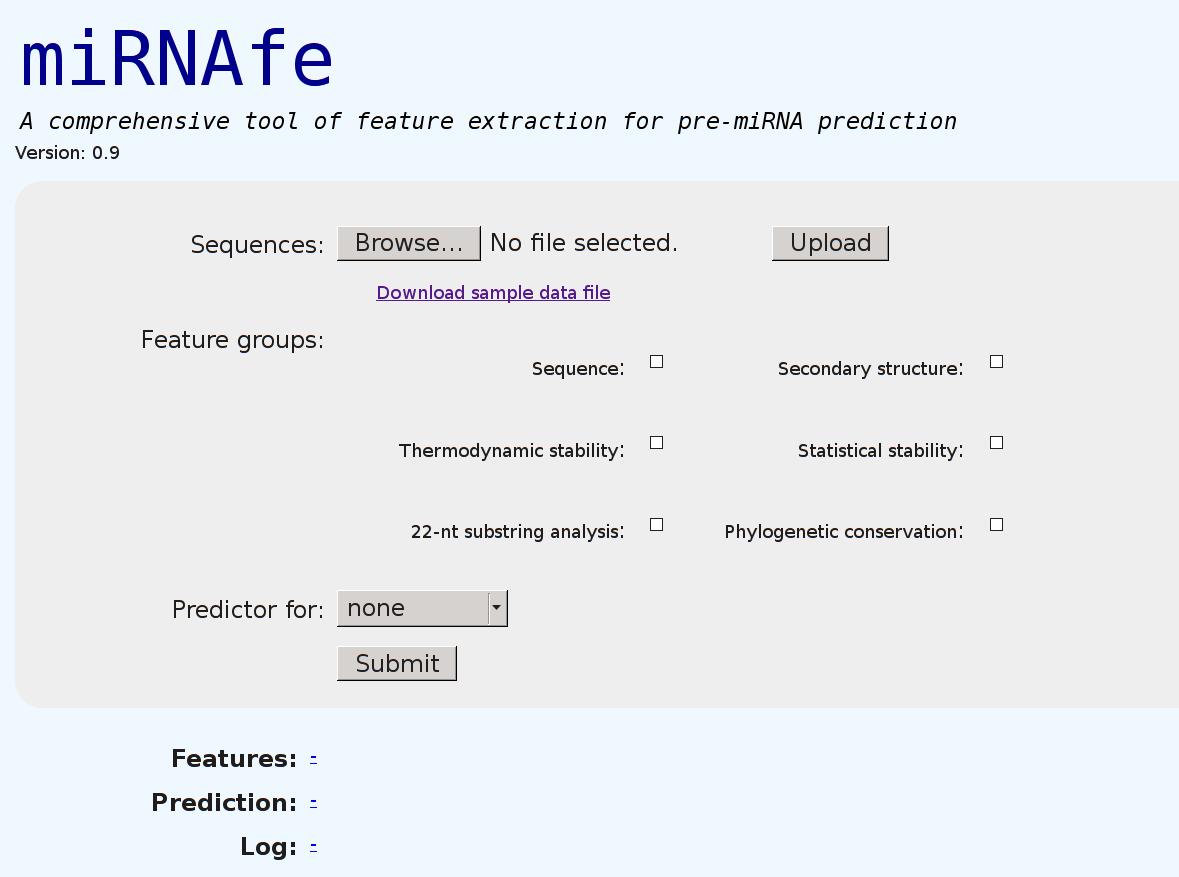
\includegraphics[width=\textwidth]{screenshot.png}
 \caption{Web interface of miRNAfe after analyzing some sample sequences}
 \label{fig:screenshot}
\end{figure}

\section{Validation of the feature extraction processes}
In order to validate all feature extraction scripts, several sequences were analyzed with miRNAfe and with the software of the original authors, and the
outputs have been compared. The sequences used in this validation step were the well-known pre-miRNAs: ppa-mir-101, hsa-mir-34a, hsa-mir-7-1, hsa-let-7a-1,
hsa-let-7a-3 and hsa-let-7b3. These sequences were selected randomly with the sole purpose of validating the feature extraction functions. The software used to
validate the features extraction were MiRFinder \citep{Huang07}, miPred \citep{Jiang07} and microPred \citep{Rukshan09}. MiRNAfe validates the extracted
features by comparison with the reference software, when available. In most cases, however, the original scripts were not available and reference results were
obtained directly from data with already extracted features, and compared with the results of miRNAfe. In all tests performed, the results were always
consistent to those of the original papers.

The validation process was automated with a script that is distributed together with the source code of the tool. This script prints on screen the results of
each test, the reference value and the software that was used to obtained it. This can also be used to make tests and re-validate the results of each function
after making improvements or alternative implementations of the algorithms. For the statistical features, where results are not deterministic, a confidence
interval for the expected values was set according to the variance in each case. The validation error was calculated as $e = 100 \|C- E\|_{2} / \|E\|_{2}$,
where $C$ is the result calculated by miRNAfe, $E$ is the expected value (the one calculated with the software of the original author) and $||\cdot||_2$ is the
norm 2. A list with the software used for comparisons and their corresponding references are provided in the supplementary material.


\section{Acknowledgments}
This work was supported by National Scientific and Technical Research Council [PIP 2013 117], National University of Litoral [CAI+D 2011 548] and Agencia
Nacional de Promoci{\'o}n Cient{\'i}fica y Tecnol{\'o}gica (ANPCyT) [PICT 2014 2627].

\bibliographystyle{natbib}
\bibliography{mirnafe}

\end{document}
